\parindent=0em
\documentclass[11pt, oneside]{book}   						%use article, report, book
\input{Vorspann_Defi_color.tex}

\algblockdefx{Title}{EndTitle}[1][]{\textbf{#1}: }{}
\algblockdefx{ForEach}{EndForEach}[1][]{\textbf{for each} #1 \textbf{do}}{\textbf{end for}}
\algblockdefx{Atomic}{EndAtomic}{\textbf{atomically do}}{\textbf{end do}}

\title{Principles of Distributed Computing Summary}
\author{Ulla Aeschbacher}
\date{20.6.18}				%started, added section 1
\date{21.6.18}				%added section 2
\date{28.6.18}				%added section 3,4,5
\date{29.6.18}				%added section 6,7,8
\date{2.7.18}				%added section 9,10,11
\date{4.6.18}				%added section 12,13,
\date{5.6.18}				%added section 14
\date{4.8.18}				%added list of theorems, definitions, algorithms, cleaned up definitions of those

\iffalse

\begin{algorithm}
\caption{\tb{}}\label{}
\begin{algorithmic}[1]
\end{algorithmic}
\end{algorithm}


\begin{center}
\begin{tikzpicture}
\end{tikzpicture}\\[1em]
\captionof{figure}{Half-Cleaner}
\end{center}

\fi

\usepackage{thmtools}

\makeatletter
\def\ll@mythm{%
  \protect\numberline{\csname the\thmt@envname\endcsname}%
  \ifx\@empty\thmt@shortoptarg
    \thmt@thmname
  \else
    \thmt@shortoptarg
  \fi}
\def\l@thmt@mythm{} 

\def\ll@mydef{%
  \protect\numberline{\csname the\thmt@envname\endcsname}%
  \ifx\@empty\thmt@shortoptarg
    \thmt@thmname
  \else
    \thmt@shortoptarg
  \fi}
\def\l@thmt@mydef{} 
\makeatother


\begin{document}
\maketitle

\tableofcontents

\listoftheorems[ignoreall, show={mythm}]
\renewcommand\listtheoremname{List of Definitions}
\listoftheorems[ignoreall, show={mydef}]
\listofalgorithms

%%%%%%%%%%%%%%%%%%%%%%%%%%%%%%%%%%%%%%%%%%%%%%%%%%%%%%%%%%%%%%%%%%%%%%%%
%%%%%%%%%%%%%%%%%%%%%%%%%%%%%%%%%%%%%%%%%%%%%%%%%%%%%%%%%%%%%%%%%%%%%%%%
\chapter{Definitions}
%%%%%%%%%%%%%%%%%%%%%%%%%%%%%%%%%%%%%%%%%%%%%%%%%%%%%%%%%%%%%%%%%%%%%%%%
\section{General Graph Stuff}
\begin{mydef}[$BFS_v$] Performing a breadth first search at node $v$ produces spanning tree $BFS_v$. This takes time $\mc{O}(\Delta)$ using small messages.\end{mydef}
\begin{mydef}[Blue Edge] Cheapest edge that connects two subtrees. Formally:  Let $T$ be a spanning tree of the weighted graph $G$ and $T'\subseteq T$ a subgraph of $T$. The minimum weight outgoing edge $b(T')$ is the so-called blue edge of $T'$.\end{mydef}
\begin{mythm}For a given weighted graph $G$, let $T$ denote the MST and $T'$ be a fragment of $T$. Then the blue edge of $T'$ is also part of $T$.\end{mythm}
\begin{mydef}[Chromatic Number] Given an undirected graph $G=(V,E)$, the chromatic number $\chi(G)$ is the minimum number of colors to solve the vertex coloring problem.\end{mydef}
\begin{mythm}$\chi(\text{Tree}) \le 2$\end{mythm}
\begin{mydef}[Clean] A graph is clean if the nodes do not know the topology of the graph.\end{mydef}
\begin{mydef}[Coordinator Model] We have $n$ players numbered 1 to $n$, as well as an arbitrary $n$-node graph $G$. The $i^{th}$ player knows the edges incident on the $i^{th}$ node. \end{mydef}
\begin{mydef}[Degree] The number of neighbors of a vertex $v$, denoted by $\delta(v)$, is called the degree of $v$. The maximum degree in a graph $G$ defines the graph degree $\Delta(G)=\Delta$.\end{mydef}
\begin{mydef}[Diameter] The diameter of a graph is the maximum distance between two arbitrary nodes in a graph.\end{mydef}
\begin{mythm}[Lower Bound on Computing the Diameter] Any distributed algorithm $A$ that computes the diameter of a graph needs $\Omega\left(\frac{n}{\log n}\right)$ time.\end{mythm}
\begin{mydef}[Distance] The distance between two nodes $u$ and $v$ in an undirected graph $G$ is the number of hops of a minimum path between $u$ and $v$.\end{mydef}
\begin{mydef}[Graph-Familiy $\mc{G}$] We assume that $(n-2)$ can be divided by 8. We define four sets of nodes, each consisting of $q=q(n)=\frac{n-2}{4}$ nodes:
\begin{itemize}
	\item $L_0=\{l_i| i\in [q]\}$
	\item $L_1=\{l_i'| i\in [q]\}$
	\item $R_0=\{r_i| i\in [q]\}$
	\item $R_1=\{r_i'| i\in [q]\}$
\end{itemize}
We define $G'=(V',E')$ as
$$V' = L_0 \cup L_1 \cup R_0 \cup R_1 \cup \{c_L,c_R\}$$
\begin{alignat*}{3}
E' = & &\quad& \bigcup_{v\in L_0\cup L_1}\{(v,c_L)\} \\
& \cup && \bigcup_{v\in R_0\cup R_1}\{(v,c_R)\} \\
& \cup && \bigcup_{i\in [q]} \{(l_i,r_i),(l_i',r_i')\}\cup\{(c_L,c_R)\}\\
& \cup && \bigcup_{S\in \{L_0,L_1,R_0,R_1\}}\bigcup_{u\neq v\in S}\{(u,v)\}
\end{alignat*}
\begin{center}
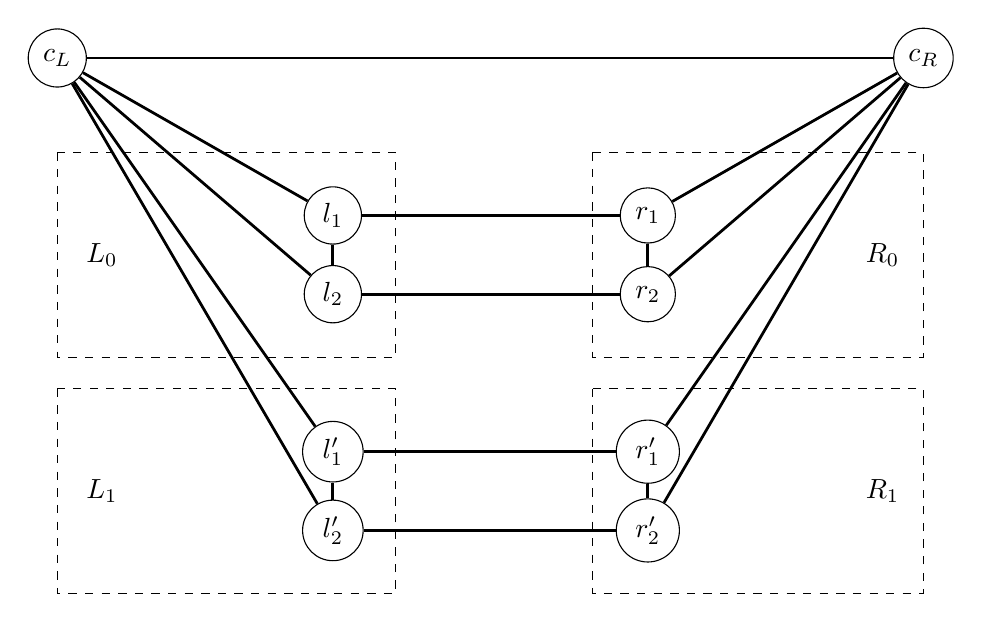
\begin{tikzpicture}
\node [circle, draw] (L) at (0,1) {$c_L$};
\draw [dashed] (0,-0.2) rectangle (4.3,-2.8) node [midway, xshift=-45pt] {$L_0$}; 
\draw [dashed] (0,-3.2) rectangle (4.3,-5.8) node [midway, xshift=-45pt] {$L_1$}; 
\node [circle, draw] (A) at (3.5,-1) {$l_1$};
\node [circle, draw] (B) at (3.5,-2) {$l_2$};
\node [circle, draw] (C) at (3.5,-4) {$l_1'$};
\node [circle, draw] (D) at (3.5,-5) {$l_2'$};
\draw [line width=1pt] (L) -- (A);
\draw [line width=1pt] (L) -- (B);
\draw [line width=1pt] (L) -- (C);
\draw [line width=1pt] (L) -- (D);
\draw [line width=1pt] (A) -- (B);
\draw [line width=1pt] (C) -- (D);

\node [circle, draw] (R) at (11,1) {$c_R$};
\draw [dashed] (6.8,-0.2) rectangle (11,-2.8) node [midway, xshift=45pt] {$R_0$}; 
\draw [dashed] (6.8,-3.2) rectangle (11,-5.8) node [midway, xshift=45pt] {$R_1$}; 
\node [circle, draw] (E) at (7.5,-1) {$r_1$};
\node [circle, draw] (F) at (7.5,-2) {$r_2$};
\node [circle, draw] (G) at (7.5,-4) {$r_1'$};
\node [circle, draw] (H) at (7.5,-5) {$r_2'$};
\draw [line width=1pt] (R) -- (E);
\draw [line width=1pt] (R) -- (F);
\draw [line width=1pt] (R) -- (G);
\draw [line width=1pt] (R) -- (H);
\draw [line width=1pt] (E) -- (F);
\draw [line width=1pt] (G) -- (H);

\draw [line width=1pt] (L) -- (R);
\draw [line width=1pt] (A) -- (E);
\draw [line width=1pt] (B) -- (F);
\draw [line width=1pt] (C) -- (G);
\draw [line width=1pt] (D) -- (H);

\end{tikzpicture}\\[1em]
\captionof{figure}{Graph $G'\in \mc{G}$ with $n=10$}
\end{center}
Family $\mc{G}$ contains any graph $G$ that is derived from $G'$ by adding any combination of edges of the for, $(l_i, l_j')$ or $(r_i,r_j')$.
\end{mydef}
\begin{mydef}[Graph Sketch] A compressed representation of the graph.\end{mydef}
\begin{mydef}[Labeling Scheme] A labeling scheme consists of an encoder $e$ and a decoder $d$. The encoder $e$ assigns to each node $v$ a label $e(v)$. The decoder $d$ receives the labels of the nodes in question and returns an answer to some query. The largest size (in bits) of a label assigned to a node is called the label size of the labeling scheme.\end{mydef}\hfill\\

\begin{mythm}[Upper Bound for Adjacency in Trees]It is possible to assign labels of size $2\log n$ bits to nodes in a tree, so that for every pair $u,v$ of nodes it is easy to tell whether they are adjacent or not, just by looking at their labels.\end{mythm}
\begin{mythm}[Lower Bound for Adjacency in General Graphs] Any labeling scheme for adjacency in general graphs has a label size of at least $\Omega(n)$ bits.\end{mythm}
\begin{mydef}[Maximal Independent Set (MIS)] Given a graph $G=(V,E)$, a set of vertices $S\subseteq V$ is called a MIS, if it satisfies the following properties:
\begin{itemize}
	\item The set $S$ is an independent set meaning that no two vertices $u,v\in S$ are adjacent.
	\item The set $S$ is maximal meaning that for each node $v\notin S$ there exists a neighbor $u$ of $v$ such that $u\in S$.
\end{itemize}\end{mydef}
\begin{mydef}[Maximum Matching] A matching is a set of edges $M\subseteq E$ such that no two of the edges on $M$ share an end-point. A matching is maximal if we cannot add any edge to $M$ without violating the property that we have a matching.\end{mydef}
\begin{mythm}In any graph, any maximal matching has size at least $\efrac{2}$ of the maximum matching.\end{mythm}
\begin{mydef}[Minimal Spanning Tree (MST)] Given a weighted graph $G=(V,E,\omega)$, the MST of $G$ is a spanning tree $T$ minimizing $\omega(T)$, where $\omega(G')=\sum_{e\in G'}\omega_e$ for any subgraph $G'\subseteq G$\end{mydef}
\begin{mydef}[Outgoing Edge] Let $T$ be a spanning tree of the weighted graph $G$ and $T'\subseteq T$ a subgraph of $T$. Edge $e=(u,v)$ is an outgoing edge of $T'$ if $u\in T'$  and $v\notin T'$ or vice versa.\end{mydef}
\begin{mydef}[Radius] The radius of a node $u$ is the maximum distance between $u$ and any other node in the graph. The radius of a graph is the minimum radius of any node in the graph.\end{mydef}
\begin{mydef}[Shortest Path Cover] The node set $S_i$ is a shortest path cover if $S_i$ contains a node on every shortest path of length between $2^{i-1}$ and $2^i$.\end{mydef}

%%%%%%%%%%%%%%%%%%%%%%%%%%%%%%%%%%%%%%%%%%%%%%%%%%%%%%%%%%%%%%%%%%%%%%%%
\section{Algorithms and Complexity}
\begin{mydef}[Synchronous Distributed Algorithm] In a synchronous distributed algorithm, nodes operate in synchronous rounds. In each round, each node executes the following steps: 
\begin{enumerate}
	\item Send messages to neighbors in graph (of reasonable size).
	\item Receive messages (that were sent by neighbors in step 1 of the same round)
	\item Do some local computation (of reasonable complexity)
\end{enumerate}\end{mydef}
\begin{mydef}[Asynchronous Distributed Algorithm] In the asynchronous model, algorithms are event driven. Nodes cannot access a global clock. A message sent from one node to another will arrive in finite but unbounded time.\end{mydef}
\begin{mydef}[Synchronous Time Complexity] For synchronous algorithms the time complexity is the number of rounds until the algorithm terminates.\end{mydef}
\begin{mydef}[Asynchronous Time Complexity] For asynchronous algorithms the time complexity is the number of time units from the start of the execution to its compeltion in the worst case, assuming that each message has a delay of at most one time unit.\end{mydef}
\begin{mydef}[Message Complexity] The message complexity of an algorithm is determined by the total number of messages exchanges.\end{mydef}

%%%%%%%%%%%%%%%%%%%%%%%%%%%%%%%%%%%%%%%%%%%%%%%%%%%%%%%%%%%%%%%%%%%%%%%%
\section{Vertex Coloring}
\begin{mydef}[Vertex Coloring] Given an undirected graph $G=(V,E)$, assign a color $c_v$ to each vertex $v \in V$ such that the following holds: $e=(v,w) \in E \Rightarrow c_v \neq c_w$.\end{mydef}
\begin{mydef}[$\log^*$] $$\forall x\le 2: \log^*x :=1 \qquad \forall x > 2: \log^*c:= 1+\log*(\log x)$$
This is a very slow growing function. $\log^*(10^{80}) = 5$\end{mydef}
\begin{mydef}[Cover-free Family] Given a ground set $\{1,2, \hdots, k'\}$, a family of sets $S_1,S_2,\hdots,S_k\subseteq\{1,2,\hdots k'\}$ is called a $\Delta$-cover free family if and only if for each set of indices $i_0,i_1,\hdots, i_\Delta\in \{1,2,\hdots,k\}$, we have 
	$$S_{i_0}\backslash \left(\bigcup_{j=1}^\Delta S_{i_j}\right)\neq \emptyset$$
That is, if no set in the family is a subset of the union of $\Delta$ other sets.\end{mydef}
\begin{mydef}[Sperner Family] A Sperner family is simply a 1-cover free family.\end{mydef}
\begin{mythm}For any $k$ and $\Delta$, there exists a $\Delta$-cover free family of size $k$, $S_1, S_2\hdots,S_k \subseteq\{1,2,\hdots, k'\}$, on a ground set of size $k'=\mc{O}(\Delta^2\log k)$.\end{mythm}
\begin{mydef}[$k$-ary $q$-coloring] We say $B$ is a $k$-ary $q$-coloring if for any set of ientifiers $1\le a_1<\hdots<a_{k+1}\le n$, we have the foloowing properties:
\begin{itemize}
	\item $B(a_1,\hdots, a_k)\in \{1,\hdots, q\}$
	\item $B(a_1, \hdots, a_k)\neq B(a_2,\hdots, a_{k+1})$
\end{itemize}\end{mydef}
\begin{mythm}[Lower Bound on Coloring Rooted Trees] Any deterministic algorithm for 3-coloring $n$-node directed paths needs at least $\frac{\log^*n}{2}-2$ rounds.\end{mythm}
\begin{mythm}[Lower Bound on Coloring Unrooted Trees] Any deterministic distributed algorithm $A$ that colors $n$-node trees with maximum degree $\Delta$ using less than $o(\frac{\Delta}{\log\Delta})$ colors has round complexity at least $\Omega(\log_\Delta n)$.\end{mythm}
\begin{mythm}[Upper Bound on Coloring Unrooted Trees] There is a deterministic distributed algorithm that computes a 3-coloring of any $n$-node tree in $\mc{O}(\log n)$ rounds.\end{mythm}

%%%%%%%%%%%%%%%%%%%%%%%%%%%%%%%%%%%%%%%%%%%%%%%%%%%%%%%%%%%%%%%%%%%%%%%%
\section{Distributed Sorting}
\begin{mydef}[Sorting] We choose a graph with $n$ nodes $v_1,\hdots, v_n$. Initially each node stores a value. After applying a sorting algorithm, node $v_k$ stores the $k^{th}$ smallest value.\end{mydef}
\begin{mydef}[0-1 Sorting Lemma] If an oblivious comparison.exchange algorithm sorts all inputs of 0's and 1's, then it sorts arbitrary inputs.\end{mydef}
\begin{mydef}[Node Contention] In each step of a synchronous algorithm, each node can only send and receive $\mc{O}(1)$ messages containing $\mc{O}(1)$ values, no matter how many neighbors the node has.\end{mydef}
\begin{mydef}[Comparator] A comparator is a device with two inputs $x,y$ and two outputs $x',y'$ such that $x'=\min(x,y)$ and $y'=\max(x,y)$.\end{mydef}
\begin{mydef}[Comparison Network] A comparison network consists of wires that connect comparators. Some wires are not connected to comparator outputs (input wires) and some are not connected to comparator outputs (output wires).\end{mydef}
\begin{mydef}[Sorting Network] A sorting network with width $n$ has $n$ input wires and $n$ output wires. A sorting network routes $n$ values given on the input wires through the wires and comparators of the network such that the values are sorted on the output wires.\end{mydef}
\begin{mydef}[Depth] The depth of an input wire is 0. The depth of a comparator is the maximum depth of its input wires plus one. The depth of an output wire of a comparator is the depth of the comparator. The depth of a comparison network is the maximum depth of an output wire.\end{mydef}
\begin{mydef}[Bitonic Sequence] A bitonic sequence is a sequence of numbers that first monotonically increases and then monotonically decreases or vice versa.\end{mydef}
\begin{mydef}[Distributed Counting] A distributed counter is a variable that is common to all processors in a system and that supports an atomic test-and-increment operation. The operation delivers the system's counter value to athe requesting processor and increments it.\end{mydef}

%%%%%%%%%%%%%%%%%%%%%%%%%%%%%%%%%%%%%%%%%%%%%%%%%%%%%%%%%%%%%%%%%%%%%%%%
\section{Network Decomposition}
\begin{mydef}[Weak Diameter Network Decomposition] Given a graph $G=(V,E)$, a $(\mc{C}, \mc{D})$ weak diameter network decomposition of $G$ is a partition of $G$ into vertex-disjoint graphs $G_1, \hdots, G_\mc{C}$, such that for each $i\in \{1, \hdots, \mc{C}\}$, we have the following property: the graph $G_i$ is made of a number of vertex-disjoint and mutually non-adjacent clusters $X_1, \hdots, X_l$, where each two vertices $v,u\in X_j$ have distance at most $\mc{D}$ in graph $G$. We note that we do not bound the number $l$. We refer to each subgraph $G_i$ as one block of this network decomposition.\end{mydef}
\begin{center}
\begin{tikzpicture}
\node [circle, fill = black, minimum size = 4pt] (A) at (0,0) {} ;
\node [circle, fill = black, minimum size = 4pt] (B) at (2,-1) {} ;
\node [circle, fill = black, minimum size = 4pt] (C) at (1,-2) {} ;
\node [circle, fill = black, minimum size = 4pt] (D) at (1.5,1.5) {} ;
\node [circle, fill = black, minimum size = 4pt] (E) at (4,0.5) {} ;
\node [circle, fill = black, minimum size = 4pt] (F) at (3,-3) {} ;
\node [circle, fill = black, minimum size = 4pt] (G) at (5,-2) {} ;
\node [circle, fill = black, minimum size = 4pt] (H) at (5.5,-1) {} ;
\draw [line width=1pt] (A) -- (B);
\draw [line width=1pt] (A) -- (C);
\draw [line width=1pt] (B) -- (C);
\draw [line width=1pt] (B) -- (D);
\draw [line width=1pt] (B) -- (E);
\draw [line width=1pt] (B) -- (F);
\draw [line width=1pt] (C) -- (D);
\draw [line width=1pt] (D) -- (E);
\draw [line width=1pt] (E) -- (F);
\draw [line width=1pt] (F) -- (G);
\draw [line width=1pt] (G) -- (H);
\draw [mred, rounded corners=5mm] (1,1.2) -- (1,2.2) node [anchor=south]{$G_1$}-- (4.5,0.8) -- (4.5, -0.2) -- cycle;
\draw [mgreen, rounded corners=10mm] (-1,1) node {$G_2, X_1$}-- (3, -0.5) -- (1,-3) -- cycle;
\draw [mgreen, rounded corners=5mm] (4.3,-2.5) -- (5.3,-2.5) -- (6.2,-0.5) node [anchor=south west]{$G_2,X_2$} -- (5.2,-0.5) -- cycle;
\draw [mblue,anchor=north] (3,-3) circle (18pt) node [anchor=north, yshift=-18pt]{$G_3$};
\end{tikzpicture}\\[1em]
\captionof{figure}{$(3,1)$ Weak Diameter Network Decomposition}
\end{center}
\begin{mydef}[Strong Network Decomposition] Given a graph $G=(V,E)$, a $(\mc{C}, \mc{D})$ strong diameter network decomposition of $G$ is a partition of $G$ into vertex-disjoint graphs $G_1, \hdots, G_\mc{C}$ such that for each $i\in \{1, \hdots, \mc{C}\}$, we have the following property: each connected component of $G_i$ has diameter at most $\mc{D}$.\end{mydef}

%%%%%%%%%%%%%%%%%%%%%%%%%%%%%%%%%%%%%%%%%%%%%%%%%%%%%%%%%%%%%%%%%%%%%%%%
\section{Wireless Protocols}
\begin{mydef}[Initialization] At the end of the initialization, the $n$ nodes should have the IDs $\{1,\hdots, n\}$.\end{mydef}
\begin{mydef}[Non-Uniform Network] The nodes know things about the network, e.g. how many nodes there are in total.\end{mydef}
\begin{mydef}[Uniform Network] The nodes know nothing about the network.\end{mydef}
\begin{mydef}[Collision Detection (CD)] Two or more nodes transmitting concurrently is called interference. In a system with collision detection, a receiver can distinguish interference from nobody transmitting. In a system without collision detection, a receiver cannot distinguish the two cases.\end{mydef}
\begin{mythm}[Lower Bound on Leader Election]Any uniform protocol that elects a leader with probability of at least $1-\efrac{2^t}$ must run for at least $t$ time slots.\end{mythm}
\begin{mythm}[Uniform Asynchronous Wakeup with CD] If nodes wake up in an arbitrary (worst-case) way, any algorithm may take $\Omega(\frac{n}{\log n})$ time slots until a single node can successfully transmit.\end{mythm}

%%%%%%%%%%%%%%%%%%%%%%%%%%%%%%%%%%%%%%%%%%%%%%%%%%%%%%%%%%%%%%%%%%%%%%%%
%%%%%%%%%%%%%%%%%%%%%%%%%%%%%%%%%%%%%%%%%%%%%%%%%%%%%%%%%%%%%%%%%%%%%%%%
\chapter{Math Stuff}
%%%%%%%%%%%%%%%%%%%%%%%%%%%%%%%%%%%%%%%%%%%%%%%%%%%%%%%%%%%%%%%%%%%%%%%%
\begin{mythm}$$\alpha > 1: \quad 1+\frac{\log(\alpha-1)}{2} \le \log \alpha$$\end{mythm}
\begin{mythm}[Chernoff Bound] Suppose $X_1, \hdots, X_\eta$ are independent random variables taking values in $[0,1]$. Let $X=\sum_{i=1}^lX_i$ denote their sum and let $\mu=\mb{E}[X]$ denote the sum's expected value. For any $0\le \delta \le 1$ it holds
	$$Pr[X < (1-\delta)E[X]] \le e^{-\frac{\delta^2}{2}E[X]}$$
and for $\delta > 0$
	$$Pr[X\ge (1+\delta) E[X]] \le e^{-\frac{\min\{\delta, \delta^2\}}{3}E[X]}$$
\end{mythm}
\begin{mydef}[With High Probability] Some probabilistic event is said to occur with high probability if it happens with a probability $p\ge 1-\efrac{n^c}$, where $c$ is a constant.\end{mydef}
\begin{mythm}[Booles Inequality] For a countable set of events $E_1, E_2, E_3, \hdots$ we have
	$$Pr\left[\bigcup_iE_i\right] \le \sum_i Pr[E_i]$$
\end{mythm}
\begin{mythm}[Markovs Inequality] If $X$ is any random variable and $a>0$ then
	$$Pr\left[\abs{X}\ge a\right] \le \frac{E[X]}{a}$$
\end{mythm}
\begin{mythm}For all $n\in \mb{N}$ and $\abs{t} \le n$ we have 
	$$e^t\left(1-\frac{t^2}{n}\right)\le \left(1+\frac{t}{n}\right)^n\le e^t$$
Note that:
	$$\lim_{n\to \infty}\left(1+\frac{t}{n}\right)^n = e^t$$
\end{mythm}
\begin{mythm}For all $p,q$ such that $0<p<1$ and $k\ge 1$ we have
	$$1-p\le \left(1-\frac{p}{k}\right)^k$$
\end{mythm}

%%%%%%%%%%%%%%%%%%%%%%%%%%%%%%%%%%%%%%%%%%%%%%%%%%%%%%%%%%%%%%%%%%%%%%%%
%%%%%%%%%%%%%%%%%%%%%%%%%%%%%%%%%%%%%%%%%%%%%%%%%%%%%%%%%%%%%%%%%%%%%%%%
\chapter{Algorithms}
%%%%%%%%%%%%%%%%%%%%%%%%%%%%%%%%%%%%%%%%%%%%%%%%%%%%%%%%%%%%%%%%%%%%%%%%
\section{Vertex Coloring}
\textbf{\tb{Goal: Color the nodes of a graph with as few different colors as possible.}}
\begin{algorithm}
\caption{\tb{Greedy Sequential}}\label{greedyseq}
\begin{algorithmic}[1]
\While{there is an uncolored vertex $v$}
	\State Color $v$ with the minimal color that does not conflict with already colored neighbors
\EndWhile
\end{algorithmic}
\end{algorithm}
\begin{mythm}[Algorithm \ref{greedyseq}] Terminates in $n$ steps. Uses at most $\Delta+1$ colors.\end{mythm}

\begin{algorithm}
\caption{\tb{Reduce}}\label{reduce}
\begin{algorithmic}[1]
\State Assume that initially all nodes have IDs
\ForEach [node $v$]
	\State Send ID to all neighbors
	\State Receive IDs of all neighbors
	\While{node $v$ has an uncolored neighbor with higher ID}
		\State Send "undecided" to all neighbors
		\State Receive decisions from neighbors
	\EndWhile
	\State Choose the smallest admissible free color
	\State Send color choice to all neighbors
\EndForEach
\end{algorithmic}
\end{algorithm}
\begin{mythm}[Algorithm \ref{reduce}] Time complexity $n$. Uses at most $\Delta +1$ colors.\end{mythm}

\begin{algorithm}[H]
\caption{\tb{Slow Tree Coloring}}\label{slowtree}
\begin{algorithmic}[1]
\State Color the root with 0, the root sends 0 to its children
\ForEach[node $v$]
	\If{node $v$ receives a message $c_p$ from parent}
		\State Choose color $c_v=(1-c_p)\mod 2$
		\State Send $c_v$ to children
	\EndIf
\EndForEach
\end{algorithmic}
\end{algorithm}
\begin{mythm}[Algorithm \ref{slowtree}] Time complexity is the height of the tree.\end{mythm}

\begin{algorithm}
\caption{\tb{6-color}}\label{scolor}
\begin{algorithmic}[1]
\State Assume that initially the nodes have IDs (labels) of size $\log n$ bits
\State The root assigns to itself the label 0
\ForEach[other node $v$]
	\State Send own color $c_v$ to all children
	\Repeat
		\State Receive color $c_p$ from parent
		\State Interpret $c_v$ and $c_p$ as bit-strings
		\State Let $i$ be the index of the smallest bit where $c_v$ and $c_p$ differ
		\State The new label is $i$ (as bit-string) followd by the $i^{th}$ bit of $c_v$
		\State Send $c_v$ to all children
	\Until{$c_w\in \{0, \hdots, 5\}$ for all nodes $w$}
\EndForEach
\end{algorithmic}
\end{algorithm}
\begin{myremark}Examples: \\[0.5em]
\begin{tabular}{l r c r c r}
	grandparent: & 0010\tr{1}10000 & $\to$ & 1\tr{0}010 & $\to$ & \\
	parent: & 1\tg{0}10\tr{0}10000 & $\xrightarrow{5,0}$ & 0\tr{1}01\tg{0} & $\xrightarrow{3,1}$ & 111\\
	child: & 0\tg{1}10010000 & $\xrightarrow{8,1}$ & 1000\tg{1} & $\xrightarrow{0,1}$ & 001
\end{tabular}

\begin{tabular}{l r c r }
	grandparent: & 110\tr{0}101101 & $\to$ & \\
	parent: & 101\tr{1}101101 & $\xrightarrow{6,1}$ & 1101 \\
	child: & 001\tr{0}101101 & $\xrightarrow{6,0}$ & 1100
\end{tabular}\end{myremark}
\begin{mythm}[Algorithm \ref{scolor}] Terminates in $\log^*(n+c)$ time.\end{mythm}

\begin{algorithm}[H]
\caption{\tb{3-color}}\label{tcolor}
\begin{algorithmic}[1]
\State Assume that initially the nodes have IDs (labels) of size $\log n$ bits
\State The root assigns to itself the label 0
\ForEach[other node $v$]
	\State Send own color $c_v$ to all children
	\Repeat
		\State Receive color $c_p$ from parent
		\State Interpret $c_v$ and $c_p$ as bit-strings
		\State Let $i$ be the index of the smallest bit where $c_v$ and $c_p$ differ
		\State The new label is $i$ (as bit-string) followd by the $i^{th}$ bit of $c_v$
		\State Send $c_v$ to all children
	\Until{$c_w\in \{0, \hdots, 5\}$ for all nodes $w$}
\EndForEach
\ForEach[node $v$]
	\For{$x=5,4,3$}
		\ForEach[node $v$]
			\State Recolor $v$ with the color of the parent
			\State Root choses new, different color from $\{0,1,2\}$
		\EndForEach
		\If{$c_v=x$}
			\State Choose smallest admissible new color $c_v\in \{0,1,2\}$
		\EndIf
	\EndFor
\EndForEach
\end{algorithmic}
\end{algorithm}
\begin{mythm}[Algorithm \ref{tcolor}] Terminates in time $\mc{O}(\log^*n)$\end{mythm}
\begin{myremark}A fast tree-coloring with only 2 colors is more than exponentially more expensive than coloring with 3 colors.
\end{myremark}
\begin{myremark}A general graph with constant degree $\Delta$ can be colored with $\Delta + 1$ colors in $\mc{O}(\log^*n)$ time.
\end{myremark}

\begin{algorithm}
\caption{\tb{Linial}}\label{linial}
\begin{algorithmic}[1]
\State Given a $n$-coloring of the graph.
\While {there are more than $\mc{O}(\Delta^2 \log\Delta)$ colors}
	\State Given a $k$-coloring $\phi_{old}$ of a graph with maximum degree $\Delta$.
	\ForEach[node $v$ of old color $\phi_{old}(v)=q, q\in \{1, \hdots, k\}$]
		\State Use set $S_q\subseteq\{1, \hdots, k'\}$ in the cover free family as its color-set
		\State Set new color $\phi_{new}(v)=q', q'\in S_q$ such that $q'$ is not in the color-set of any of the neighbors
	\EndForEach
\EndWhile
\end{algorithmic}
\end{algorithm}
\begin{mythm}[Algorithm \ref{linial}] Needs $\mc{O}(\log^* n)$ rounds to compute a $\mc{O}(\Delta^2\log \Delta)$-coloring.\end{mythm}

\begin{algorithm}
\caption{\tb{Color Reduction}}\label{colorred}
\begin{algorithmic}[1]
\ForEach[node $v$]
	\State $c_v = v$
\EndForEach
\For{$v=\Delta+2$ \textbf{ to } $n$}
	\State $c_v =\min(\{1,\hdots, \Delta +1\}\backslash \{c_u|(u,v)\in E\})$
\EndFor
\end{algorithmic}
\end{algorithm}

\begin{algorithm}
\caption{\tb{Kuhn-Wattenhofer}}\label{kw}
\begin{algorithmic}[1]
\ForEach[node $v$] in parallel
	\State $c_v = v$
\EndForEach
\While{$k> \Delta +1$}
	\State Divide colors into bins of size $2(\Delta +1)$
	\State Let each bin be denoted as $G_i =(V_i,E_i)$
	\For{i} in parallel
		\State Color Reduction($G_i$)
		\State $k = k- \Delta + 1$
	\EndFor
\EndWhile
\end{algorithmic}
\end{algorithm}
\begin{mythm}[Algorithm \ref{kw}] Needs $\mc{O}(\Delta\lceil\log(\frac{k}{\Delta+1})\rceil)$ rounds to compute a $(\Delta+1)$-coloring.\end{mythm}

\begin{mythm}By first performing Algorithm \ref{linial} and then Algorithm \ref{kw} we can achieve a $(\Delta+1)$-coloring in $\mc{O}(\Delta\log\Delta + \log^*n)$ rounds.\end{mythm}

\begin{algorithm}
\caption{\tb{Luby MIS}}\label{luby}
\begin{algorithmic}[1]
\While {set is not maximal}
	\ForEach[node $v$]
		\State $v$ picks a random number $r_v\in [0,1]$ and sends it to its neighbors.
	\EndForEach
	\ForEach[node $v$]
		\If {$r_v>r_u$ for all neighbors $u$ of $v$}
			\State $v$ joins MIS set $S$
			\State $v$ informs its neighbors
			\State $v$ and all its neighbors are removed from the graph
		\EndIf
	\EndForEach
\EndWhile
\end{algorithmic}
\end{algorithm}
\begin{mythm}[Algorithm \ref{luby}] Computes a MIS in $\mc{O}(\log n)$ rounds with high probability.\end{mythm}\hfill\\
\begin{mythm}Given a distributed algorithm $\mc{A}$ that computes a MIS of any $n$-node graph in $T(n)$ rounds, there is a distributed algorithm $\mc{B}$ that computes a $(\Delta+1)$-coloring of any $n$-node graph with maximum degree $\Delta$ in $T(n(\Delta+1))$ rounds. Short outline: Compute MIS $S_i$, color with color $i$, remove $S_i$ from graph, repeat.\end{mythm}

\begin{algorithm}
\caption{\tb{Coloring Unrooted Trees}}\label{unrooted}
\begin{algorithmic}[1]
\Statex \textit{Step 1, takes $\mc{O}(\log n)$ iterations}
\State $T_1=T$
\State $L_1 = \{v\in T_1|degree(v)\le 2\}$
\While {layer $L_{i+1}$ still get nodes}
	\State $T_{i+1} = T_i\backslash L_i$
	\State $L_{i+1} = \{v\in T_{i+1}|degree(v)\le 2\}$
	\State $i=i+1$
\EndWhile
\State $T = T[\bigcup_{j=1}^l L_j]$
\Statex
\Statex \textit{Step 2, takes $\mc{O}(\log^*n)$ rounds}
\ForEach[$T[L_i]$]
	\State 3-color $T[L_i]$ with Algorithm \ref{tcolor} to get schedule colors
\EndForEach
\Statex
\Statex \textit{Step 3, takes $l\cdot3 = \mc{O}(\log n)$ rounds}
\For {$i=l$ \textbf{until} $i=1$}
	\For {$q\in \{1,2,3\}$}
		\State Have final coloring of $T[\bigcup_{j=i+1}^l L_j]$
		\State Pick a final color in $\{1,2,3\}$ for all the vertices in $L_i$ with schedule color $q$.
	\EndFor
\EndFor
	
\end{algorithmic}
\end{algorithm}

%%%%%%%%%%%%%%%%%%%%%%%%%%%%%%%%%%%%%%%%%%%%%%%%%%%%%%%%%%%%%%%%%%%%%%%%
\section{Edge Coloring}
\textbf{\tb{Goal: Color the edges of a graph with as few different colors as possible.}}
\begin{algorithm}[H]
\caption{\tb{Edge-Coloring}}\label{edgecolor}
\begin{algorithmic}[1]
\Statex \textit{Part 1}
\State Orient the graph $G$, so that each edge goes from lower ID to higher ID
\ForEach[node $v$]
	\State Number outgoing edges of $v$
\EndForEach
\State Define $F_i$ as vertices and edges which are numbered $i^{th}$ by their starting point.
\State $F_i$ is an oriented pseudo-forest (each component has at most one circle)
\Statex
\Statex \textit{Part 2}
\ForEach[$F_i$] in parallel
	\State Compute a 3-vertex-coloring with Algorithm \ref{tcolor}.
	\State These are the schedule-colors of $F_i$.
\EndForEach
\Statex
\Statex \textit{Part 3}
\For {$k\in \{1,2,3\}$}
	\State Let $E_k^i$ be the set of $F_i$-edges whose parent endpoint is colored with color $k$. 
	\State These edges form vertex-disjoint stars.
	\ForEach[star centered at node $v$ with nodes $u_1, \hdots, u_l$] in parallel
		\State $v$ learns colors of edges adjacent to $u_1,\hdots, u_l$
		\State $v$ computes edge-colors for edges $(v,u_1),\hdots,(v,u_l)$. There will always be a color available from colors $\{1,2\Delta-1\}$.
	\EndForEach
\EndFor
\end{algorithmic}
\end{algorithm}
\begin{mythm}[Algorithm \ref{edgecolor}] Needs $\mc{O}(\Delta +\log^* n)$ rounds to compute a $(2\Delta-1)$-edge-coloring.\end{mythm}

%%%%%%%%%%%%%%%%%%%%%%%%%%%%%%%%%%%%%%%%%%%%%%%%%%%%%%%%%%%%%%%%%%%%%%%%
\section{Tree Construction Algorithms}
\textbf{\tb{Goal: Construct trees from graphs.}}
\begin{algorithm}
\caption{\tb{Flooding}}\label{flooding}
\begin{algorithmic}[1]
\State The source (root) sends the message to all neighbors
\ForEach[node $v$ upon receiving the message the first time]
	\State Forward the message to all other neighbors
\EndForEach
\State Upon later receiving the message again, a node can discard the message
\end{algorithmic}
\end{algorithm}
\begin{mythm}[Algorithm \ref{flooding}] Time complexity $radius(root)$. Message complexity $m$ where $m=\abs{E}$ is the number of edges (if the nodes do not know the topology) or $n-1$ (if the nodes know the topology).\end{mythm}

\begin{algorithm}
\caption{\tb{Echo}}\label{echo}
\begin{algorithmic}[1]
\ForEach[leaf $v$]
	\State Send a message to its parent
\EndForEach
\ForEach[not-leaf $u$ upon receiving a message from a child]
	\State Send message to its parent
\EndForEach
\end{algorithmic}
\end{algorithm}
\begin{mythm}[Algorithm \ref{echo}] Time complexity is determined by the depth of the spanning tree. Message complexity $n-1$. Together with flooding: 
$$\begin{tabular}{l | l l}
	flooding/echo & synchronous & asynchronous\\
	\hline
	time complexity & $2\cdot radius(root)$ & $n$\\
	message complexity & $4m + n \le 5m$ & $c\cdot m$
\end{tabular}$$\end{mythm}

\begin{algorithm}
\caption{\tb{Dijkstra BFS}}\label{dijkstra}
\begin{algorithmic}[1]
\State Phase $p=1$, treee $T$ which is the root plus all direct neighbors of the root
\Repeat
	\State Root starts phase $p$ by broadcasting "start $p$" within $T$
	\ForEach[leaf node $u$ upon receiving "start $p$"]
		\State Send a "join $p+1$" message to all neighbors it has not communicated with yet.
		\State Collect all answers of neighbors then start echo back to the root
	\EndForEach
	\ForEach[node $v$ upon receiving "join $p+1$"]
		\If{$v$ not in $T$}
			\State Reply with "ack" and become new leaf of tree $T$ at level $p+1$
		\Else
			\State Reply with "nack"
		\EndIf
	\EndForEach
	\State When echo process terminates at root, root sets new phase $p=p+1$
\Until {there was no new node detected}
\end{algorithmic}
\end{algorithm}
\begin{mythm}[Algorithm \ref{dijkstra}] Time complexity $\mc{O}(D^2)$. Message complexity $\mc{O}(m+n\cdot D)$ where $D$ is the diameter of the graph.\end{mythm}

\begin{algorithm}
\caption{\tb{Bellman-Ford BFS}}\label{bellmanford}
\begin{algorithmic}[1]
\State $u$ stores $d_u$ = distance from $u$ to the root. Initially $d_{root}=0$ and $d_u=\infty $ for all other nodes $u$.
\State root starts by sending "1" to all neighbors
\If{node $u$ receives message "$y$" with $y<d_u$ from neighbor $v$}
	\State $u$ sets $d_u := y$
	\State $u$ sends "$y+1$" to all neighbors except $v$
\EndIf
\end{algorithmic}
\end{algorithm}
\begin{mythm}[Algorithm \ref{bellmanford}] Time complexity $\mc{O}(D)$. Message complexity $\mc{O}(n\cdot m)$, where $D$ is the diameter of the graph.\end{mythm}
\begin{myremark}Algorithm \ref{dijkstra} has better message complexity and Algorithm \ref{bellmanford} has better time complexity. The current best algorithm has time complexity $\mc{O}(D\cdot \log^3n)$ and message complexity $\mc{O}(m+n \log^3n)$.
\end{myremark}

\begin{algorithm}
\caption{\tb{Gallager-Humblet-Spira (GHS)}}\label{ghs}
\begin{algorithmic}[1]
\State Each node is root of its own fragment.
\Repeat
	\State All nodes learn fragment IDs of their neighbors
	\State Root of each fragment uses flooding/echo in its fragment to determine the blue edge $b=(u,v)$ of the fragment.
	\State Root sends a message to node $u$. While forwarding the message from root to $u$, all parent-child relations are inverted.
	\State $u$ sends merge request over the blue edge $b=(u,v)$ 
	\If {$v$ also sent a merge request over the same blue edge $b=(u,v)$}
		\State $u$ or $v$ (with smaller ID) is new fragment root
		\State $b$ is directed accordingly
	\Else
		\State $v$ is new parent of $u$
	\EndIf
	\State newly elected root node $u$ or $v$ informs all nodes in its fragment about its identity using flooding/echo
\Until all nodes are in the same fragment
\end{algorithmic}
\end{algorithm}
\begin{mythm}[Algorithm \ref{ghs}] Time complexity $\mc{O}(n\log n)$. Message complexity $\mc{O}(m\log n)$.\end{mythm}

%%%%%%%%%%%%%%%%%%%%%%%%%%%%%%%%%%%%%%%%%%%%%%%%%%%%%%%%%%%%%%%%%%%%%%%%
\section{Shared Objects on Trees}
\textbf{\tb{Goal: Manage access to a common object in a tree.}}
\begin{algorithm}
\caption{\tb{Shared Object: Centralized Solution}}\label{centralized}
\begin{algorithmic}[1]
\Statex\textit{Initialization: }{Shared objects stored at root node $r$ of a spanning tree of the network graph. All nodes know their parent.}
\Statex
\Statex\textit{Accessing Object} {by node $v$}
	\State $v$ sends request up the tree
	\State Request atomically processed by root $r$
	\State Result sent down the tree to node $v$
\end{algorithmic}
\end{algorithm}
\begin{myremark}Algorithm \ref{centralized} suffers whem a single node accesses the shared object repeatedly.
\end{myremark}

\begin{algorithm}
\caption{\tb{Shared Object: Home-Based Solution}}\label{homebased}
\begin{algorithmic}[1]
\Statex\textit{Initialization:} {An object has a home base node that is known to every node. All requests are touted through the home base.}
\Statex
\Statex\textit{Accessing Object} {by node $v$}
	\State $v$ acquires a lock at the home base, receives object
\end{algorithmic}
\end{algorithm}
\begin{myremark}Algorithm \ref{homebased} suffers from the triangular routing problem: If two close-by nodes access the object in turns, all the traffic is routed through the potentially far away home-base.
\end{myremark}

\begin{algorithm}[H]
\caption{\tb{Shared Object: Arrow}}\label{arrow}
\begin{algorithmic}[1]
\Statex\textit{Initialization:} {We are given a rooted spanning tree. Each node has a pointer to its parent, the root $r$ is its own parent. The object is initially stored at $r$. For all nodes $v: v.successor:=null, v.wait:=false$.}
\Statex
\Statex\textit{Start Find Request at Node $u$}
\Atomic
	\State $u$ sends "find by $u$ message to parent node
	\State $u.parent := u$
	\State $u.wait := true$
\EndAtomic
\Statex
\Statex\textit{Upon $w$ receiving "Find by $u$" Message from Node $v$}
\Atomic
	\If{$w.parent \neq w$}
		\State $w$ sends "find by $u$" message to parent
		\State $w.parent := v$
	\Else
		\State $w.parent := v$
		\If{not $w.wait$}
			\State Send variable to $u$
		\Else
			\State $w.successor := u$
		\EndIf
		\EndIf
\EndAtomic
\Statex
\Statex\textit{Upon $w$ Receiving Shared Object}
\State Perform operation on shared object
\Atomic
	\State $w.wait := false$
	\If{$w.successor \neq null$}
		\State Send variable to $w.successor$
		\State $w.successor := null$
	\EndIf
\EndAtomic
\end{algorithmic}
\end{algorithm}\hfill\\
\begin{mythm}[Algorithm \ref{arrow}] For one "find" operation in a concurrent (meaning there can be many find requests at the same time) setting.
\begin{itemize}
	\item Asynchronous: Time complexity $D$. Message complexity $D$ where $D$ is the diameter of the spanning tree. 
	\item Synchronous setting: Message complexity $\mc{O}(\log\abs{S}\cdot m^*)$ where $S$ is the set of nodes initiating a "find" operation and $m^*$ the message complexity of an optimal algorithm on the tree.
\end{itemize}\end{mythm}

%not covered in lecture, thus not part of exam
%\begin{algorithm}
%\caption{\tb{Shared Object: Read/Write Caching}}\label{readwrite}
%\begin{algorithmic}[1]
%\Statex Nodes can either read or write the shared object. Assume that access to object is sequential. 
%\Statex Nodes store three items: a parent pointer pointing to one of the neighbors, a cache bit for each edge and potentially a copy of the object.
%\Statex Initially the object is stored at a single node $u$. All parent pointers point towards $u$ and all cache bits are false.
%\Statex When initiating a read, a message follows the arrow until it reaches a cached version of the object. Then a copy of the object is cached along the path back to the initiating node and the cache bits on the visited edges are set to true.
%\Statex A write at $u$ writes the new value locally, then searches a first node with a copy. Delete copy and follow in parallel all edges that have the cache flag set. Point the pointer towards $u$ now and remove the cache flags.
%\end{algorithmic}
%\end{algorithm}
%\begin{mythm}[Algorithm \ref{readwrite}] Message complexity is 3-competitve (at most a factor 3 worse than the optimum). When adding concurrent writes, it becomes 4-competitive.\end{mythm}

%%%%%%%%%%%%%%%%%%%%%%%%%%%%%%%%%%%%%%%%%%%%%%%%%%%%%%%%%%%%%%%%%%%%%%%%
\section{Shared Objects on Cliques}
\textbf{\tb{Goal: Manage access to a common object in a clique.}}
\begin{algorithm}
\caption{\tb{Shared Object: Pointer Forwarding}}\label{pointerforward}
\begin{algorithmic}[1]
\Statex\textit{Initialization: }{Object is stored at root $r$ of a precomputed spanning tree $T$.}
\Statex
\Statex\textit{Accessing object} by node $v$
\State Follow parent pointers to current root $r$ of $T$
\State Send object from $r$ to $u$
\State $r.parent := u, \quad u.parent := u$
\end{algorithmic}
\end{algorithm}
\begin{mythm}[Algorithm \ref{pointerforward}] In the worst case (always first node of linked list that acquires object): Time complexity $n$. Message complexity $n$. If not FIFO, can even be unbounded.\end{mythm}

\begin{algorithm}
\caption{\tb{Shared Object: Ivy}}\label{ivy}
\begin{algorithmic}[1]
\Statex\textit{Initialization: }{Object is stored at root $r$ of a precomputed spanning tree $T$.}
\Statex
\Statex\textit{Start Find Request at Node $u$}
\State $u$ send "find by $u$" message to parent node
\State $u.parent := u$
\Statex
\Statex\textit{Upon $v$ receiving "Find by $u$" Message}
\If{$v.parent = v$}
	\State Send object to $u$
\Else
	\State Send "find by $u$" message to $v.parent$
\EndIf
$v.parent := u$ 
\end{algorithmic}
\end{algorithm}
\begin{mythm}[Algorithm \ref{ivy}] For one "find" operation and if initial tree is a star, time complexity is $\log n$, where $n$ is the number of processors.\end{mythm}

%%%%%%%%%%%%%%%%%%%%%%%%%%%%%%%%%%%%%%%%%%%%%%%%%%%%%%%%%%%%%%%%%%%%%%%%
\section{Distributed Sorting}
\textbf{\tb{Goal: Have the $k^{th}$ node store the $k^{th}$-smallest value.}}
\begin{algorithm}
\caption{\tb{Odd/Even Sort}}\label{oddeven}
\begin{algorithmic}[1]
\State Given an array of $n$ nodes $(v_1,\hdots, v_n)$, each storing a value
\Repeat
	\State Compare and exchange the values at nodes $i$ and $i+1$, $i$ odd
	\State Compare and exchange the values at nodes $i$ and $i+1$, $i$ even
\Until {done}
\end{algorithmic}
\end{algorithm}
\begin{mythm}[Algorithm \ref{oddeven}] Sorts correctly in $n$ steps.\end{mythm}

\begin{algorithm}[H]
\caption{\tb{Shearsort}}\label{shearsort}
\begin{algorithmic}[1]
\State We are given a mesh with $m$ rows and $m$ columns, $m$ even, $n=m^2$.
\Repeat { alternating odd/even phases}
	\If{is odd phase}
		\ForEach[row]
			\If{row is odd}
				\State Sort row such that small values move to the left
			\Else
				\State Sort row such that small values move to the right
			\EndIf
		\EndForEach
	\Else
		\State Sort columns such that small values move up
	\EndIf
\Until done
\end{algorithmic}
\end{algorithm}
\begin{mythm}[Algorithm \ref{shearsort}] Sorts $n$ values in $2\cdot m\cdot (\log n +1)= \sqrt{n}(\log n+1)$ time in snake-like order.\end{mythm}

\begin{algorithm}
\caption{\tb{Half Cleaner}}\label{halfcleaner}
\begin{algorithmic}[1]
\State Comparison network of depth 1
\State Compare wire $i$ with wire $i+\frac{n}{2}$ for $i=1, \hdots, \frac{n}{2}$.
\end{algorithmic}
\end{algorithm}
\begin{center}
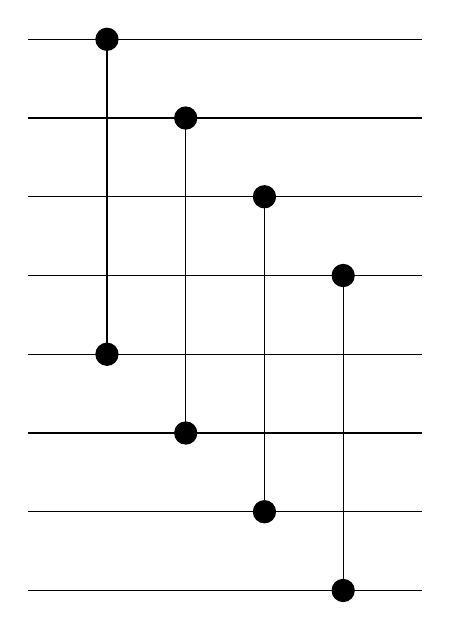
\begin{tikzpicture}
\foreach \x in {1,...,8} {\draw (0,\x) -- (5,\x);}
\draw [fill = black] (1,4) circle (4pt);
\draw (1,4) -- (1, 8);
\draw [fill = black] (1,8) circle (4pt);
\draw [fill = black] (2,3) circle (4pt);
\draw (2,3) -- (2, 7);
\draw [fill = black] (2,7) circle (4pt);
\draw [fill = black] (3,2) circle (4pt);
\draw (3,2) -- (3, 6);
\draw [fill = black] (3,6) circle (4pt);
\draw [fill = black] (4,1) circle (4pt);
\draw (4,1) -- (4, 5);
\draw [fill = black] (4,5) circle (4pt);
\end{tikzpicture}\\[1em]
\captionof{figure}{Half-Cleaner (HC)}
\end{center}
\begin{mythm}[Algorithm \ref{halfcleaner}] Fed a bitonic sequence, it cleans either the upper or the lower half of the $n$ wires. The other half is bitonic.\end{mythm}
\begin{algorithm}
\caption{\tb{Merger}}\label{merger}
\begin{algorithmic}[1]
\State A merger is a comparison network of depth 1.
\State Compare wire $i$ with wire $n-i+1$ for $i=1, \hdots, \frac{n}{2}$
\end{algorithmic}
\end{algorithm}
\begin{center}
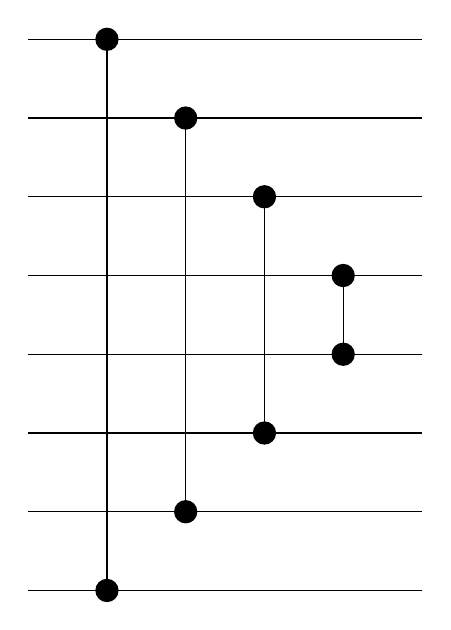
\begin{tikzpicture}
\foreach \x in {1,...,8} {\draw (0,\x) -- (5,\x);}
\draw [fill = black] (1,1) circle (4pt);
\draw (1,1) -- (1, 8);
\draw [fill = black] (1,8) circle (4pt);
\draw [fill = black] (2,2) circle (4pt);
\draw (2,2) -- (2, 7);
\draw [fill = black] (2,7) circle (4pt);
\draw [fill = black] (3,3) circle (4pt);
\draw (3,3) -- (3, 6);
\draw [fill = black] (3,6) circle (4pt);
\draw [fill = black] (4,4) circle (4pt);
\draw (4,4) -- (4, 5);
\draw [fill = black] (4,5) circle (4pt);
\end{tikzpicture}\\[1em]
\captionof{figure}{Merger}
\end{center}
\begin{mythm}[Algorithm \ref {merger}] Fed two sorted sequences of width $\frac{n}{2}$, it gives two bitonic sequences of width $\frac{n}{2}$.\end{mythm}

\begin{algorithm}
\caption{\tb{Bitonic Sequence Sorter}}\label{bss}
\begin{algorithmic}[1]
\State Consists of a half-cleaner of width $n$ and then two bitonic sequence sorters of width $\frac{n}{2}$ each.
\State A bitonic sequence sorter of width 1 is empty.
\end{algorithmic}
\end{algorithm}
\begin{center}
\begin{tikzpicture}
\draw [anchor = east, -{Stealth}] (-2,2) node {Bitonic}-- (0,2) ;
\draw (0,0) rectangle (7,4);
\draw (3.5, 4) node [anchor=south, yshift=0.2cm] {BSS};
\draw (0.5,0.5) rectangle (3.5, 3.5) node [midway] {HC};
\draw (4,0.5) rectangle (6.5, 1.75) node [midway] {BSS};
\draw (4,2.25) rectangle (6.5, 3.5) node [midway] {BSS};
\draw [anchor = west, -{Stealth}] (7,2) -- (9,2) node {Sorted};
\end{tikzpicture}\\[1em]
\captionof{figure}{Bitonic Sequence Sorter (BSS)}
\end{center}
\begin{mythm}[Algorithm \ref{bss}] Sorts bitonic sequences in depth $\log n$.\end{mythm}


\begin{algorithm}
\caption{\tb{Merging Network}}\label{mergingnet}
\begin{algorithmic}[1]
\State Consists of a merger of width $n$ followed by two bitonic sequence sorters fo width $\frac{n}{2}$ each.
\end{algorithmic}
\end{algorithm}
\begin{center}
\begin{tikzpicture}
\draw [anchor = east, -{Stealth}] (-2,1) node {Sorted}-- (0,1);
\draw [dashed] (-4,2) -- (0,2);
\draw [anchor = east, -{Stealth}] (-2,3) node {Sorted}-- (0,3);
\draw (0,0) rectangle (7,4);
\draw (3.5, 4) node [anchor=south, yshift=0.2cm] {MN};
\draw (0.5,0.5) rectangle (3.5, 3.5) node [midway] {Merger};
\draw (4,0.5) rectangle (6.5, 1.75) node [midway] {BSS};
\draw (4,2.25) rectangle (6.5, 3.5) node [midway] {BSS};
\draw [anchor = west, -{Stealth}] (7,2) -- (9,2) node {Sorted};
\end{tikzpicture}\\[1em]
\captionof{figure}{Merging Network (MN)}
\end{center}
\begin{mythm}[Algorithm \ref{mergingnet}] Merges two sorted input sequences of length $\frac{n}{2}$ into one sorted sequence of length $n$.\end{mythm}

\begin{algorithm}
\caption{\tb{Batcher's Sorting Network}}\label{batcher}
\begin{algorithmic}[1]
\State Consists of two batcher sorting networks of width $\frac{n}{2}$ each followed by a merging network of width $n$.
\State A batcher sorting network of width 1 is empty.
\end{algorithmic}
\end{algorithm}
\begin{center}
\begin{tikzpicture}
\draw [anchor = east, -{Stealth}] (-2,2) node {Anything}-- (0,2);
\draw (0,0) rectangle (7,4);
\draw (3.5, 4) node [anchor=south, yshift=0.2cm] {BSN};
\draw (0.5,0.5) rectangle (3.5, 1.75) node [midway] {BSN};
\draw (0.5,2.25) rectangle (3.5, 3.5) node [midway] {BSN};
\draw (4,0.5) rectangle (6.5, 3.5) node [midway] {MN};
\draw [anchor = west, -{Stealth}] (7,2) -- (9,2) node {Sorted};
\end{tikzpicture}\\[1em]
\captionof{figure}{Batcher Sorting Network (BSN)}
\end{center}
\begin{mythm}[Algorithm \ref{batcher}] Sorts an arbitrary sequence of length $n$ in depth $\mc{O}(\log^2 n)$.\end{mythm}

\begin{center}
\begin{tikzpicture}
\foreach \x in {1,...,8} {\draw (0,\x) -- (12,\x);} 				% horizontal lines

\draw [anchor = south] (2.5, 8.5) node{2 $\times$ Batcher};
\draw [dashed] (0.5,0.5) rectangle (4.4, 4.4);
\draw [dashed] (0.5,4.6) rectangle (4.4, 8.5);
\foreach \x in {1,...,8} {\draw [fill = black](1,\x) circle (4pt);} 	
\foreach \x in {1,4,5,8} {\draw [fill = black](2,\x) circle (4pt);}
\foreach \x in {2,3,6,7} {\draw [fill = black](3,\x) circle (4pt);}
\foreach \x in {1,...,8} {\draw [fill = black](4,\x) circle (4pt);} 
\draw (2,1) -- (2,4);
\draw (2,5) -- (2,8);
\draw (3,2) -- (3,3);
\draw (3,6) -- (3,7);

\draw [anchor = south, color=mgreen] (8, 10.5) node{MN};
\draw [dashed, color=mgreen] (4.5,0.3) rectangle (11.6, 10.5);
\draw [anchor = south] (6.5, 8.5) node{Merger};
\draw [dashed] (4.6,0.5) rectangle (8.4, 8.5);
\foreach \x in {1,8} {\draw [fill = black](5,\x) circle (4pt);}
\foreach \x in {2,7} {\draw [fill = black](6,\x) circle (4pt);}
\foreach \x in {3,6} {\draw [fill = black](7,\x) circle (4pt);}
\foreach \x in {4,5} {\draw [fill = black](8,\x) circle (4pt);}
\draw (5,1) -- (5,8);
\draw (6,2) -- (6,7);
\draw (7,3) -- (7,6);
\draw (8,4) -- (8,5);

\draw [anchor = south, color=mblue] (10, 9.5) node{BSS};
\draw [dashed, color=mblue] (8.5,0.4) rectangle (11.5, 9.5);
\draw [anchor = south] (9.5, 8.5) node{HC};
\draw [dashed] (8.6,0.5) rectangle (10.4, 8.5);
\foreach \x in {2,4,6,8} {\draw [fill = black](9,\x) circle (4pt);}
\foreach \x in {1,3,5,7} {
	\draw [fill = black](10,\x) circle (4pt);
	\draw (1,\x) -- (1,\x+1);
	\draw (4,\x) -- (4,\x+1);
	\draw (11,\x) -- (11,\x+1);
}
\draw (9,2) -- (9,4);
\draw (9,6) -- (9,8);
\draw (10,1) -- (10,3);
\draw (10,5) -- (10,7);

\draw [anchor = south] (11, 8.5) node{BSS};
\draw [dashed] (10.6,0.5) rectangle (11.4, 8.5);
\foreach \x in {1,...,8} {\draw [fill = black](11,\x) circle (4pt);}
\end{tikzpicture}\\[1em]
\captionof{figure}{Batcher for width 8}
\end{center}

%%%%%%%%%%%%%%%%%%%%%%%%%%%%%%%%%%%%%%%%%%%%%%%%%%%%%%%%%%%%%%%%%%%%%%%%
\section{Centralized Maximum Matching}
\textbf{\tb{Goal: Use a few local computations to approximate the size of the maximum matching.}}

\begin{algorithm}
\caption{\tb{Random Greedy Maximal Matching Algorithm}}\label{rgmma}
\begin{algorithmic}[1]
\ForEach [edge $e$]
	\State Pick random number $r_e\in[0,1]$
\EndForEach
\For {edge $e$ with lowest $r_e$ \textbf{until} edge $e$ with highest $r_e$}
	\State Add $e$ to the matching $M$ if no neighbor $e'$ of $e$ with lower $r_{e'}$ is already in $M$.
\EndFor
\end{algorithmic}
\end{algorithm}

\begin{algorithm}
\caption{\tb{Centralized Maximal Matching Algorithm}}\label{cmma}
\begin{algorithmic}[1]
\State We want to find out if $e$ is in the matching $M$ or not.
\State Determine random value $r_e$ and all $r_e'$ for all neighbors $e'$ of $e$.
\ForEach [$e'$ with $r_e' < r_e$]
	\State Recursively find out if they are in the matching $M$
\EndForEach
\If {none of the edges $e'$ with $r_e' < r_e$ is in the matching $M$}
	\State $e$ is in the matching $M$
\EndIf
\end{algorithmic}
\end{algorithm}
\begin{mythm}[Algorithm \ref{cmma}] The expected query complexity of the algorithm for an arbitrary edge $e$ is at most $2^{\mc{O}(\Delta)}$.\end{mythm}
\begin{mythm}[Approximating the Size of the Maximal Matching] Pick a set $S$ of $k$ random chosen nodes. The fraction of theses nodes that are matched in $M$ is an unbiased estimator of the fraction of vertices that are matched in $M$. Thus:
$$ \abs{M} \approx \frac{n}{2\abs{S}}\sum_{s\in S}1_{(\text{vertex } s \text{ matched in }M)}$$
For any certainty parameter $\delta\in [0,0.25]$ and any precision parameter $\epsilon > 0$, suppose we choose a set $S$ of $k=\frac{20\cdot\Delta\cdot\log1/\delta}{\epsilon^2}$ at random. Then this function provides a $(1+\epsilon)$ approximation of the size of the maximal matching with probability at least $1-\delta$.\\
The overall expected query complexity for checking a set $S$ of nodes to see whether they are matched in $M$ or not is at most $\abs{S}\cdot \Delta \cdot 2^{\mc{O}(\Delta)} = \abs{S}\cdot 2^{\mc{O}(\Delta)}$\end{mythm}

%%%%%%%%%%%%%%%%%%%%%%%%%%%%%%%%%%%%%%%%%%%%%%%%%%%%%%%%%%%%%%%%%%%%%%%%
\section{Network Decomposition}
\textbf{\tb{Goal: Compute a network decomposition with which we can solve a wide range of problems.}}
\begin{algorithm}
\caption{\tb{Weak Network Decomposition}}\label{weakdecomp}
\begin{algorithmic}[1]
\For{$i=1$ \textbf{until} $\mc{C}$}
	\ForEach[node $u$]
		\State Pick random radius $r_u$ with $Pr[r_u=y] = \epsilon(1-\epsilon)^{y-1}$ for $\epsilon\in (0,1)$
		\State The ball of node $u$ are the vertices within distance $r_u$ of $u$. 
	\EndForEach
	\ForEach[node $v$]
		\State Let $Center(v) = u'$ be the smallest-identifier node whose ball contains $v$.
	\EndForEach
	\State Define $G_i$ by letting all nodes with the same center define one cluster
	\State Discard nodes who are at the boundary fo their cluster
\EndFor
\end{algorithmic}
\end{algorithm}
\begin{mythm}[Algorithm \ref{weakdecomp}] Computes a $(\mc{C}, \mc{D})$ weak diameter network decomposition of any $n$-node graph $G$, for $\mc{C}=\mc{O}(\log n)$ and $\mc{D} = \mc{O}(\log n)$, in $\mc{O}(\log^2 n)$ rounds with high probability.\end{mythm}
\begin{mythm}Provided a $(\mc{C}, \mc{D})$ weak diameter network decomposition of a graph $G$, we can compute a $\Delta+1$ coloring of $G$ in $\mc{O}(\mc{C}\mc{D})$ rounds.\end{mythm}

%%%%%%%%%%%%%%%%%%%%%%%%%%%%%%%%%%%%%%%%%%%%%%%%%%%%%%%%%%%%%%%%%%%%%%%%
\section{Wireless Protocols}
\textbf{\tb{Goal: Do initialization and leader election in a wireless network where there is interference if two or more nodes transmit at the same time.}}
\begin{algorithm}
\caption{\tb{Slotted ALOHA}}\label{aloha}
\begin{algorithmic}[1]
\ForEach[node $v$] 
	\Repeat
		\State Transmit with probability $\efrac{n}$
	\Until{One node has transmitted alone}
\EndForEach
\State This node is now the leader.
\end{algorithmic}
\end{algorithm}
\begin{mythm}[Algorithm \ref{aloha}] Allows a node to transmit alone and thus become the leader after expected time $e$.\end{mythm}

\begin{algorithm}
\caption{\tb{Non-Uniform Initialization}}\label{nonuniform}
\begin{algorithmic}[1]
\Repeat
	\State Elect a leader $v$ using Algorithm \ref{aloha}.
	\State $v$ gets the next free number and leaves the process.
\Until {No nodes are left}
\end{algorithmic}
\end{algorithm}
\begin{mythm}[Algorithm \ref{nonuniform}] Initializes $n$ nodes in $\mc{O}(e\cdot n)$ time slots.\end{mythm}

\begin{algorithm}[H]
\caption{\tb{Uniform Initialization with CD}}\label{uniformcd}
\begin{algorithmic}[1]
\State $nextID = 0$
\ForEach[node $v$]
	\State $myBitstrings = ""$
	\State $bitstringsToSplit = [""]$
	\While {$bitstringsToSplit$ is not empty}
		\State $b=bitstringsToSplit.pop()$
		\Repeat
			\If{$b=myBitstring$}
				\State Choose $r$ uniformly at random from $\{0,1\}$
				\State For the next two timeslots, transmit in slot $r$, listen in the other
			\Else
				\State For the next two timeslots, listen on both
			\EndIf
		\Until{There was at least 1 transmission on both slots}
		\If {$b=myBitstring$}
			\State $myBitstring = myBitstring+r$
		\EndIf
		\For{$r\in\{0,1\}$}
			\If{some node $u$ transmitted alone in slot $r$}
				\State Node $u$ gets ID $nextId$ and becomes passive
				\State $nextId=nextId +1$
			\Else
				\State $bitstringsToSplit.push(b+r)$
			\EndIf
		\EndFor
	\EndWhile
\EndForEach
\end{algorithmic}
\end{algorithm}
\begin{mythm}[Algorithm \ref{uniformcd}] Initializes $n$ nodes in $\mc{O}(n)$ time slots.\end{mythm}

\begin{algorithm}
\caption{\tb{Uniform Initialization without CD}}\label{uniform}
\begin{algorithmic}[1]
\State Let node $l$ be the leader and $S$ the set of nodes which want to transmit.
\State Split every time slot from Algorithm \ref{uniformcd} into two time slots.
\State \textit{First timeslot:} nodes in set $S$ transmits
\State \textit{Second timeslot:} nodes in set $S\cup \{l\}$ transmit
\State This gives the nodes sufficient information to distinguish the different cases. See Table \ref{noisesilencetable} for the details.
\State Thus Algorithm \ref{uniformcd} works also without CD
\end{algorithmic}
\end{algorithm}

\newpage
\begin{center}
\begin{tabular}{l | c | c}
	& nodes in $S$ transmit & nodes in $S\cup \{l\}$ transmit\\
	\hline
	$\abs{S}=0$ & $\times$ & \checkmark \\
	$\abs{S}=1, S=\{l\}$ & \checkmark & \checkmark\\
	$\abs{S}=1, S\neq\{l\}$ & \checkmark & $\times$\\
	$\abs{S}\ge 2$ & $\times$ & $\times$
\end{tabular}
\captionof{table}{Distinguishing between noise and silence: \checkmark stands for a successful transmission, $\times$ for noise/silence}\label{noisesilencetable}
\end{center}

\begin{algorithm}
\caption{\tb{Uniform Leader Election}}\label{uniformleader}
\begin{algorithmic}[1]
\ForEach[node $v$]
	\For{$k=1, 2,3,\hdots$}
		\For{$i=1$ \textbf{until} $c\cdot k$}
			\State Transmit with probability $p=\efrac{2^k}$
			\If Node $v$ was the only node which transmitted
				\State $v$ becomes the leader
				\State \textbf{break}
			\EndIf
		\EndFor
	\EndFor
\EndForEach
\end{algorithmic}
\end{algorithm}
\begin{mythm}[Algorithm \ref{uniformleader}] Elects a leader with high probability in $\mc{O}(\log^2 n)$ time slots if $n$ is not known.\end{mythm}

\begin{algorithm}
\caption{\tb{Uniform Leader Election with CD}}\label{uniformleadercd}
\begin{algorithmic}[1]
\ForEach[node $v$]
	\Repeat
		\State Transmit with probability $\efrac{2}$
		\If At least one node transmitted
			\State All nodes that did not transmit quit the protocol
		\EndIf
	\Until {One node transmits alone}
\EndForEach
\end{algorithmic}
\end{algorithm}
\begin{mythm}[Algorithm \ref{uniformleadercd}] Elects a leader with high probability in $\mc{O}(\log n)$ time slots if we have collision detection.\end{mythm}

\begin{algorithm}[H]
\caption{\tb{Fast Uniform Leader Election with CD}}\label{fastuniformleadercd}
\begin{algorithmic}[1]
\Statex\textit{Phase 1}
\State $i=1$
\Repeat
	\State $i=2i$
	\State Transmit with probability $\efrac{2^i}$
\Until {No node transmitted}
\Statex
\Statex\textit{Phase 2}
\State $l=\frac{i}{2}$
\State $u=i$
\While {$l+1 < u$}
	\State $j=\lceil\frac{l+u}{2}\rceil$
	\State Transmit with probability $\efrac{2^j}$
	\If {No node transmitted}
		\State $u=j$
	\Else
		\State $l=j$
	\EndIf
\EndWhile
\Statex
\Statex\textit{Phase 3}
\State $k=u$
\Repeat
	\State Transmit with probability $\efrac{2^k}$
	\If{No node transmitted}
		\State $k=k-1$
	\Else
		\State $k=k+1$
	\EndIf
\Until{Exactly one node transmitted}
\end{algorithmic}
\end{algorithm}
\begin{mythm}[Algorithm \ref{fastuniformleadercd}] With probability at least $1-\frac{\log\log n}{\log n}$ we find a leader in time $\mc{O}(\log\log n)$.\end{mythm}

%%%%%%%%%%%%%%%%%%%%%%%%%%%%%%%%%%%%%%%%%%%%%%%%%%%%%%%%%%%%%%%%%%%%%%%%
\section{Computing the Diameter}
\textbf{\tb{Goal: Compute the diameter $\Delta$ of the network, so that we can use flooding/echo to solve everything in time $\mc{O}(\Delta)$.}}
\begin{algorithm}[H]
\caption{\tb{Compute All Pairs Shortes Path (APSP)}}\label{apsp}
\begin{algorithmic}[1]
\State Assume we hace leader node $l$
\State Compute $BFS_l$ of leader $l$
\State Send a pebble $P$ to traverse $BFS_l$ in a depth-first-search way
\While {$P$ traverses $BFS_l$}
	\If{$P$ visits a new node $v$}
		\State Immediately start $BFS_v$ from node $v$
		\State Pebble $P$ waits one time slot
	\EndIf
\EndWhile
\end{algorithmic}
\end{algorithm}
\begin{mythm}[Algorithm \ref{apsp}] Computes APSP in time $\mc{O}(n)$.\end{mythm}

%%%%%%%%%%%%%%%%%%%%%%%%%%%%%%%%%%%%%%%%%%%%%%%%%%%%%%%%%%%%%%%%%%%%%%%%
\section{Minimal Spanning Tree}
\textbf{\tb{Goal: Compute minimum spanning tree (MST) in a model, where the maximum number of bits that a computer can send is $\mc{O}(\log n)$.}}

\begin{algorithm}
\caption{\tb{Finding the Minimum Weight Outgoing Edge (MWOE)}}\label{mwoe}
\begin{algorithmic}[1]
\ForEach[Component $S_i$]
	\If {$\abs{S_i} \le \sqrt{n}$}
		\ForEach[node $v$]
			\State Compute smallest weight outgoing edge with weight $c(v)$
		\EndForEach
		\State Perform Convergecast on the BFS tree of $S_i$
		\State Leader $s_i$ now knows the overall MWOE
		\State $s_i$ broadcasts the MWOE and the random bit $t(S_i)$ to all nodes of $S_i$
	\Else
		\State There are at most $\sqrt{n}$ of these components
		\State We can handle these components by performing their communications on the BFS of the whole graph $G$ simultaneously.
	\EndIf
\EndForEach
\end{algorithmic}
\end{algorithm}

\begin{algorithm}[H]
\caption{\tb{Boruvska's MST}}\label{boruvska}
\begin{algorithmic}[1]
\State Start with each node being a separate component of the forest.
\Repeat
	\ForEach[component $S_i$ with leader node $s_i$]
		\State Compute random $t(S_i)\in \{0,1\}$
		\State Find the MWOE of the component with Algorithm \ref{mwoe}
		\If{$t(S_i)==1$}
			\State Suggest to merge with the component on the other end of the MWOE
		\Else 
			\State Accept incoming suggested merge-edges from component $S_j$
			\State $s_i$ becomes leader of the new merged part
		\EndIf
		\If{$t(S_i)==1$}
			\State\textit{Learn ID of new leader}
			\State The endpoint $e_i$ that was merged on knows the ID
			\If{$\abs{S_i}\le \sqrt{n}$}
				\State Do it directly inside the component in $\mc{O}(\sqrt{n})$ rounds
			\Else
				\State Broadcast it to all nodes of the graph in $\mc{O}(D+\sqrt{n})$ rounds
			\EndIf			
		\EndIf
		\State\textit{Learn size of new component}
		\If{$t(S_i)==0$}
			\State The endpoints that were merged on know the size of both components
			\If{$\abs{S_i}\le \sqrt{n}$}
				\State Compute new component size by performing converge-case
			\Else
				\State Compute new component size by doing it through the global BFS tree
			\EndIf
			\State Deliver information to all components of $S_i$
			\State Each merge-endpoint deliver the information through its own component
		\EndIf
	\EndForEach	
\Until The number of components is 1.
\end{algorithmic}
\end{algorithm}

%%%%%%%%%%%%%%%%%%%%%%%%%%%%%%%%%%%%%%%%%%%%%%%%%%%%%%%%%%%%%%%%%%%%%%%%
\section{Graph Connectivity on Graph Sketch}
\textbf{\tb{Goal: Compute the number of connected components of a graph by having each node send a local computation to a coordinator.}}
\begin{algorithm}[H]
\caption{\tb{Graph Connectivity}}\label{graphconnect}
\begin{algorithmic}[1]
\State Have coordinator and $n$ nodes
\ForEach[node $v$]
	\State Send message of size $\mc{O}(\log^4 n)$, containing $\mc{O}(\log^2n)$ many sketches of size $\mc{O}(\log^2n)$ bits each.
	\State Each sketch has $\mc{O}(\log n)$ parts, where for the $i^{th}$ part an $\mc{O}(\log n)$ bit string is generated.
	\State A random subset of the edges incident to the node is sampled, choosing each edge with probability $2^{-i}$, then the XOR of the random edge IDs over all sampled edges is stored.
\EndForEach
\Repeat
	\State The coordinator identifies an outgoing edge for every component.
	\State The coordinator runs Boruvska's Algorithm \ref{boruvska} to merge the components
\Until All components are merged.
\end{algorithmic}
\end{algorithm}

%%%%%%%%%%%%%%%%%%%%%%%%%%%%%%%%%%%%%%%%%%%%%%%%%%%%%%%%%%%%%%%%%%%%%%%%
\section{Labeling Schemes}
\textbf{\tb{Goal: Store information in the labels of the nodes so we can easily compute a function of two nodes by only looking at the labels.}}
\begin{algorithm}
\caption{\tb{Na\"ive-Distance-Labeling($T$)}}\label{naive}
\begin{algorithmic}[1]
\State Let $l$ be the label of the root $r$ in $T$
\State Let $T_1, \hdots, T_\delta$ be the sub-trees rooted at each of the $\delta$ children of $r$
\For{$i=1,\hdots, \delta$}
	\State The root of $T_i$ gets the label obtained by appending $i$ to $l$
	\State Algorithm \ref{naive}($T_i$)
\EndFor
\end{algorithmic}
\end{algorithm}
\begin{mythm}[Algorithm \ref{naive}] A label of a node $v$ corresponds to a path from $r$ to $v$ in $T$ and the nodes on the path are labeled $(l_1), (l_1,l_2), (l_1,l_2,l_3)$ and os on. The distance between $u$ and $v$ in $T$ is obtained by reconstructing the paths from $e(u)$ and $e(v)$. This takes $\mc{O}(n\log n)$.\end{mythm}

\begin{algorithm}
\caption{\tb{Heavy-Light-Decomposition($T$)}}\label{heavy}
\begin{algorithmic}[1]
\State Node $r$ is the root of $T$
\State Let $T_1, \hdots, T_\delta$ be the sub-trees rooted at each of the $\delta$ children of $r$
\State Let $T_{max}$ be the largest sub-tree in terms of numbers of nodes
\State Mark the edge $(r,T_{max})$ as heavy
\State Mark all edges to other children as light
\State Assign the names $1, \hdots, \delta-1$ to the light edges of $r$
\For {$i=1,\hdots, \delta$}
	\State Heavy-Light-Decomposition($T_i$)
\EndFor
\end{algorithmic}
\end{algorithm}
\begin{mythm}[Algorithm \ref{heavy}] We label a node in the tree by recording how to get from the root to the node. We record he number of heavy paths a node takes and also the light nodes that it takes in between. For instance, if node $u$ can be reached by first taking 2 heavy edges, the the $7^{th}$ light edge, the 3 heavy edges , then the light edges 1 and 4, the label assigned to $u$ would be $(2,7,3,1,4)$. This takes $\mc{O}(\log^2n)$.\end{mythm}

\begin{algorithm}
\caption{\tb{Hub-Labeling}}\label{hublabel}
\begin{algorithmic}[1]
\For{$i=1, \hdots, \log D$}
	\State Compute the shortes path cover $S_i$
\EndFor
\ForEach[$v\in V$]
	\State Let $F_i(v)$ be the set $S_i\cap B(v, 2^i)$, where $B(v,2^i)$ are the nodes within the ball of radius $2^i$ around $v$
	\State Let $F(v)$ be the set $F_1(v), F_2(v),\hdots$
	\State The label of $v$ consists of the nodes in $F(v)$, with their distance to $v$
\EndForEach
\end{algorithmic}
\end{algorithm}
\begin{mythm}[Algorithm \ref{hublabel}] The decoder can scan through both labels in parallel in time $\mc{O}(h\log n\log \Delta)$, where $h$ is the so-called highway dimension of $G$, defined as $h=\max_{i,v}F_i(v)$. $h$ is conjured to be small for road networks where this algorithm is used. In practice, this algorithm is still too slow.\end{mythm}


\end{document}  